\RequirePackage{plautopatch}
\documentclass[aspectratio=169, dvipdfmx, 8pt, notheorems, uplatex]{beamer}
\usepackage{docmute}
\usepackage{mypackage}

\title[]{$(\infty,1)$圏の理論のモデルについて}
\subtitle{}
\author[第5回 すうがく徒のつどい]{よの}
\date{2024年3月31日}

\begin{document}
\maketitle

\begin{frame}
  \frametitle{}
  \tableofcontents
\end{frame}

\section{1圏から高次圏へ}

\begin{frame}
  \frametitle{$1$圏}

  \begin{definition}[$1$圏]
    次の条件を満たすクラスの組$\C = (\Ob(\C),\Mor(\C))$を$1$圏($1$-category)という. 
    \begin{itemize}
      \item 合成の存在性 
      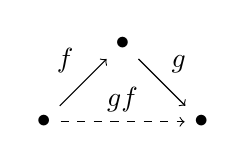
\begin{tikzpicture}[auto,->]
        \node (0) at (0,0) {$\bullet$};
        \node (1) at (1,1) {$\bullet$};
        \node (2) at (2,0) {$\bullet$};
        \draw (0) -- node {$f$} (1);
        \draw (1) -- node {$g$} (2);
        \draw[dashed] (0) -- node {$gf$} (2);
      \end{tikzpicture}
      と恒等射の存在性
      \begin{tikzpicture}[auto]
        \node (0) at (0,0) {$\bullet$};
        \node (1) at (1.5,0) {$\bullet$};
        \draw[double,dashed] (0) -- node {$\id$} (1); 
      \end{tikzpicture}
      \item 恒等射公理
      \[
      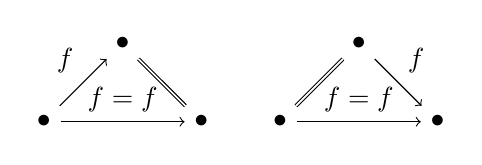
\begin{tikzpicture}[auto]
        \node (0) at (0,0) {$\bullet$};
        \node (1) at (1,1) {$\bullet$};
        \node (2) at (2,0) {$\bullet$};

        \node (3) at (3,0) {$\bullet$};
        \node (4) at (4,1) {$\bullet$};
        \node (5) at (5,0) {$\bullet$};

        \draw[->] (0) -- node {$f$} (1);
        \draw[double] (1) -- node {$\id$} (2);
        \draw[->] (0) -- node {$f\id=f$} (2);

        \draw[double] (3) -- node {$\id$} (4);
        \draw[->] (4) -- node {$f$} (5);
        \draw[->] (3) -- node {$\id f=f$} (5);
      \end{tikzpicture}
      \]
      \item 結合性公理
      \[
      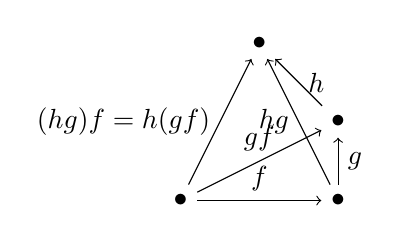
\begin{tikzpicture}[->]
        \node (0) at (0,0) {$\bullet$};
        \node (1) at (2,0) {$\bullet$};
        \node (2) at (2,1) {$\bullet$};
        \node (3) at (1,2) {$\bullet$};
        \draw (0) -- node[above] {$f$} (1);
        \draw (1) -- node[right] {$g$} (2);
        \draw (0) -- node[left] {$(hg)f=h(gf)$} (3);
        \draw (0) -- node[above] {$gf$} (2);
        \draw (1) -- node[left] {$hg$} (3);
        \draw (2) -- node[right] {$h$} (3);
      \end{tikzpicture}
      \]
    \end{itemize}
  \end{definition}

\end{frame}

\begin{frame}
  \frametitle{$2$圏}

  $1$射の間に「$2$射」が存在するような圏の例を挙げる. 

  \begin{example}
    \begin{itemize}
      \item 小圏の圏$\Cat$における$1$射(関手$F,G : \C \to \D$)の間には, 自然変換$F \Rightarrow G$が存在する. 
      \item 位相空間の圏$\Top$における1射(連続写像$f,g : X \to Y$)の間には, ホモトピー$f \Rightarrow g$が存在する. 
    \end{itemize}
  \end{example}

  このような圏は$1$圏として扱うと不都合が生じることがある. 

  \begin{remark}
    $\Cat$における次の図式の可換性は$H=GF$を意味している.
    \[
    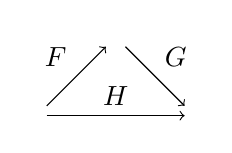
\begin{tikzpicture}[auto,->]
      \node (0) at (0,0) {$\C$};
      \node (1) at (1,1) {$\D$};
      \node (2) at (2,0) {$\E$};
      \draw (0) -- node {$F$} (1);
      \draw (1) -- node {$G$} (2);
      \draw (0) -- node {$H$} (2);
    \end{tikzpicture}
    \]
    しかし, 関手は「自然同型を除いて一意」に定義されるべきであり, 自然同型の違いは許すべきであった. 
  \end{remark}

  $\Cat$では, $1$圏が持っていない「$2$射(=$1$射の間の射)」の構造まで考える必要がある. 

\end{frame}

\begin{frame}
  \frametitle{高次の射の可逆性}

  $1$射だけでなく, $2$射($1$射の間の射)が存在するような圏を$2$圏($2$-category)という. 
  
  より一般に, $n$射までの構造を持つような圏を$n$圏($n$-category)という. 

  \begin{remark}
    $\Cat$を$1$圏としてみなすことの不都合さは見たが, $2$射としてすべての自然変換をとることも不自然である. 
    \footnote{
      関手は「自然同型の違いを除いて」一致するべきであって, 「自然変換の違いを除いて」考えることはほとんどない. 
    }
    
    つまり, この図式の可換性は「関手の一致」や「自然変換の存在」ではなく, 「自然同型の存在」を意味するべきである.     
    \[
    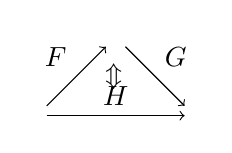
\begin{tikzpicture}[auto,->]
      \node (0) at (0,0) {$\C$};
      \node (1) at (1,1) {$\D$};
      \node (2) at (2,0) {$\E$};
      \node (star) at (1,0.5) {\rotatebox{90}{$\Leftrightarrow$}};
      \draw (0) -- node {$F$} (1);
      \draw (1) -- node {$G$} (2);
      \draw (0) -- node {$H$} (2);
    \end{tikzpicture}
    \]
  \end{remark}

  $\Cat$は$1$圏としてはtightすぎる一方で, 一般の自然変換まで考えることはlooseすぎる. 

  \begin{example}
    $\Top$における$2$射はホモトピーであったが, これは自然に可逆である. (逆向きのホモトピーを考えればよい.)

    更に, ホモトピーのホモトピー(3射)なども考えれるが, これらはすべて可逆である. 
  \end{example}

\end{frame}

\begin{frame}
  \frametitle{$(n,k)$圏および$(\infty,k)$圏}

  多くの高次圏では高次の射は可逆なので, ある$k$射以降がすべて可逆であるような$n$圏が重要である. 
  
  \begin{definition}[$(n,k)$圏]
    $(k+1)$射以降の射がすべて可逆であるような$n$圏を$(n,k)$圏($(n,k)$-category)という.
  \end{definition}

  \begin{example}
    \begin{itemize}
      \item 通常の亜群は$(1,0)$圏である. 
      \item 通常の圏は$(1,1)$圏である. 
      \item $\Cat$や$\Top$は$(2,1)$圏である(とみなす). 
    \end{itemize}
  \end{example}

  $(n,k)$圏の定義において, $n \to \infty$としたものが$(\infty,k)$圏である. 

  \begin{definition}[$(\infty,k)$圏]
    $k$を固定したときの$(n,k)$圏の集まりを$(\infty,k)$圏($(\infty,k)$-category)という. 
  \end{definition}
  
  本稿の主題は$k=1$とした$(\infty,1)$圏である. 
  つまり, $2$射以上がすべて可逆な$\infty$圏である.
\end{frame}

\section{$(\infty,1)$圏のモデル}
% \section{$(\infty,1)$圏のモデル : 位相的圏と単体的圏}

\begin{frame}
  \frametitle{位相的圏と単体的圏}

  $(\infty,1)$圏は2射以上はすべて可逆であったので, 射の集まりとして「Hom空間」を考える方法が挙げられる. 
  
  つまり, $(\infty,1)$圏は「空間」で豊穣された圏であると考える. 

  % (このとき, Hom空間における射はすべてホモトピーの違いを除いて可逆であるとみなす.)

  \begin{definition}[位相的圏]
    $\CGWH$豊穣圏
    \footnote{
      $\CGWH$はコンパクト生成弱Hausdorff位相空間の圏であり, $\Top$よりも性質がよい. 
    }
    を位相的圏(topological category)という. 
    位相的圏と位相的関手のなす圏を$\Cat_{\Top}$と表す. 
  \end{definition}

  \begin{definition}[単体的圏]
    $\sSet$豊穣圏
    \footnote{
      $\sSet$の「空間らしさ」は分かりづらいが, Dold-Kan対応や, $(\sSet)_\Quillen$と$(\Top)_\KQ$がQuillen同値であることから, イメージを掴むことができる(かも). 
    }
    を単体的圏(simplicial category)という. 
    単体的圏と単体的関手のなす圏を$\Cat_\Delta$と表す. 
  \end{definition}

  豊穣圏を用いた定義は非常に簡明であり, 豊穣圏論の一般論を使えることは利点である. 

  しかし, $(\infty,1)$関手圏の定義など, 実際に扱うことは困難な場合が多い. 
  \footnote{
    $\Cat_\Delta$上のBergnerモデル構造がCartesianモデル圏でないという理由もある. 
  }

\end{frame}

% \section{$(\infty,1)$圏のモデル : 擬圏}

\begin{frame}
  \frametitle{単体的集合}

  JoyalやLurieは「擬圏」が$(\infty,1)$圏の枠組みとして適切であることを見抜いた. 
  \footnote{
    BoardmanとVogtにより, 擬圏は弱Kan複体(weak Kan complex)として調べられていたが, これが$(\infty,1)$圏のモデルであると見抜いたのはJoyalである(はず).
  }

  \begin{definition}[単体圏]
    有限線形順序集合と狭義順序を保つ写像のなす圏を単体圏(simplex category)といい, $\Delta$と表す. 
  \end{definition}

  \begin{definition}[単体的集合]
    関手$\Delta^\myop \to \Set$を単体的集合(simplicial set)という. 
    単体的集合の圏を$\sSet$と表す. 
  \end{definition}

\end{frame}

\begin{frame}
  \frametitle{単体的集合}

  Kan拡張を用いて, 特徴的な2つの随伴が得られる. 

  \begin{remark}[ホモトピー圏をとる関手と脈体]
    埋め込み$\Delta \hookrightarrow \Cat$からKan拡張を用いることで, 次の随伴$(\h,\N)$が得られる. 
    \[
    \begin{tikzpicture}[->]
      \node (0) at (0,0) {$\Delta$};
      \node (1) at (1.5,0) {$\Cat$};
      \node (2) at (0,1.5) {$\sSet$};
      \draw[right hook->] (0) -- (1);
      \draw (0) -- node[left] {よ} (2);
      \draw (1) to[bend left=15] node[left] {$\N$} (2); % right adjoint
      \draw (2) to[bend left=15] node[right] {$\h$} (1);
    \end{tikzpicture}  
    \]
  \end{remark}

  \begin{remark}[幾何学的実現と特異単体]
    関手$\Delta[-] : \Delta \to \Top$からKan拡張を用いることで, 次の随伴$(|-|,\Sing)$が得られる. 
    \[
    \begin{tikzpicture}[->]
      \node (0) at (0,0) {$\Delta$};
      \node (1) at (1.5,0) {$\Top$};
      \node (2) at (0,1.5) {$\sSet$};
      \draw (0) -- (1);
      \draw (0) -- node[left] {よ} (2);
      \draw (1) to[bend left=15] node[below] {$\Sing$} (2); % right adjoint
      \draw (2) to[bend left=15] node[right] {$|-|$} (1);
    \end{tikzpicture}  
    \]
  \end{remark}

\end{frame}

\begin{frame}
  \frametitle{小圏の脈体}

  圏論は単体的集合の特殊な場合と思うことができる. 

  \begin{theorem}
    脈体$\N : \Cat \to \sSet$は忠実充満である. 
  \end{theorem}
  
  小圏の脈体はリフト性質で特徴づけることができる. 

  \begin{theorem}
    単体的集合$S$に対して, 次は同値である. 
    \begin{itemize}
      \item $S$はある小圏$\C$の脈体$\N(\C)$と自然同型である. 
      \item 任意の$n \geq 2$と$0<i<n$に対して, 次の図式は一意なリフトを持つ. 
      \[
      \begin{tikzpicture}
        \node (lambda) at (0,1) {$\Lambda[n,i]$};
        \node (delta) at (0,0) {$\Delta[n]$};
        \node (C) at (1,1) {$\C$};
        \draw[right hook->] (lambda) -- (delta);
        \draw[->] (lambda) -- (C);
        \draw[dashed,->] (delta) -- (C);
      \end{tikzpicture}
      \]
    \end{itemize}
  \end{theorem}
\end{frame}

\begin{frame}
  \frametitle{Kan複体}

  位相空間論におけるCW複体に対応する単体的集合のクラスを定義する. 

  \begin{definition}[Kan複体]
    任意の$n \geq 2$と$0 \leq i \leq n$に対して, 次の図式がリフト条件を持つ単体的集合$S$をKan複体(Kan complex)という. 
    \[
      \begin{tikzpicture}
        \node (lambda) at (0,1) {$\Lambda[n,i]$};
        \node (delta) at (0,0) {$\Delta[n]$};
        \node (C) at (1,1) {$\C$};
        \draw[right hook->] (lambda) -- (delta);
        \draw[->] (lambda) -- (C);
        \draw[dashed,->] (delta) -- (C);
      \end{tikzpicture}  
      \]
  \end{definition}
  
  \begin{example}
    任意の位相空間$X$に対して, 特異単体$\Sing(X)$はKan複体である.
  \end{example}

  次の意味で, 位相空間のホモトピー論は単体的集合の枠組みにおいて考えてもよい. 

  \begin{theorem}[Milnor, Giever]
    \begin{itemize}
      \item 任意の位相空間$X$に対して, $|\Sing(X)| \to X$は位相空間の弱ホモトピー同値である.
      \item 任意の単体的集合$S$に対して, $S \to \Sing(|S|)$はKan弱同値(単体的集合の弱ホモトピー同値)である.
    \end{itemize}
  \end{theorem}

\end{frame}

\begin{frame}
  \frametitle{擬圏}

  単体的集合の枠組みにおいて, 圏論は「脈体」で, 位相空間のホモトピー論は「Kan複体」によって表すことができた. 
  
  これらはともにリフト性質によって特徴づけることができたが, 2つの相違点がある. 

  \begin{block}{}
    \begin{itemize}
      \item 脈体のリフトは内部角体($0<i<n$)に対してのみだが, Kan複体のリフトは外部角体($i=0,n$)に対しても課す. 
      \item 脈体のリフトは一意だが, Kan複体のリフトは一意性を課していない. 
    \end{itemize}
  \end{block}

  脈体とKan複体の共通の一般化として, 擬圏の定義を得る. 

  \begin{definition}[擬圏]
    任意の$n \geq 2$と$0<i<n$に対して, 次のリフト条件を満たす単体的集合$\C$を擬圏(quasi-category)という. 
    \[
    \begin{tikzpicture}
      \node (lambda) at (0,1) {$\Lambda[n,i]$};
      \node (delta) at (0,0) {$\Delta[n]$};
      \node (C) at (1,1) {$\C$};
      \draw[right hook->] (lambda) -- (delta);
      \draw[->] (lambda) -- (C);
      \draw[dashed,->] (delta) -- (C);
    \end{tikzpicture}  
    \]
  \end{definition}

  \begin{example}
    \begin{itemize}
      \item 任意のKan複体は擬圏である. 
      特に, 任意の位相空間$X$に対して, 特異単体$\Sing(X)$は擬圏である. 
      \item 任意の小圏$\C$に対して, 脈体$\N(\C)$は擬圏である. 
    \end{itemize}
  \end{example}

\end{frame}

\begin{frame}
  \frametitle{擬圏は$(\infty,1)$圏のモデルである}

  擬圏において, 射の合成は「可縮な空間の選択を除いて」一意に定まる. 

  \begin{theorem}[Joyal]
    単体的集合$\C$に対して, 次は同値である. 
    \begin{itemize}
      \item $\C$は擬圏である. 
      \item 包含$\Lambda^2_1 \hookrightarrow \Delta^2$が定める単体的集合の射
      \begin{align*}
        \Fun(\Delta^2,\C) \to \Fun(\Lambda^2_1, \C)
      \end{align*}
      は自明なKanファイブレーションである.
    \end{itemize}
  \end{theorem}

  対象$x$と$y$をつなぐ射のなす単体的集合を$x$から$y$への射空間とみなす. 

  \begin{definition}[射空間]
    擬圏$\C$の対象$x,y$に対して, 単体的集合$\Hom_{\C}(x,y) := \{x\} \times_{\C} \C^{\Delta^1} \times_{\C} \{y\}$を$x$から$y$への射空間(space of morphisms)という. 
  \end{definition}

  \begin{theorem}
    擬圏$\C$の対象$x,y$に対して, 単体的集合$\Hom_{\C}(x,y)$はKan複体である. 
  \end{theorem}

  以上から, 擬圏は$(\infty,1)$圏のモデルと見ることができる. 

  % Kan複体は「空間」そのものである.
  
  % \begin{definition}[$\infty$亜群]
  %   擬圏$\C$において任意の射が同値のとき, $\C$を$\infty$亜群($\infty$-groupoid)という. 
  % \end{definition}

  % \begin{theorem}[Joyal]
  %   単体的集合$S$がKan複体であることと, $\infty$亜群であることは同値である. 
  % \end{theorem}

\end{frame}

% \section{$(\infty,1)$圏のモデル : 完備Segal空間}

\begin{frame}
  \frametitle{単体的空間}

  擬圏は脈体とKan複体に対する共通の一般化として, 単体的「集合」の枠組みにおいて拡張条件を用いて定義された. 

  一方, 完備Segal空間は単体的「空間」の枠組みにおける$(\infty,1)$圏のモデルである. 

  \begin{definition}[単体的空間]
    関手$\Delta^\myop \to \sSet$を単体的空間(simplicial space)という. 
    単体的空間の圏を$\sSpace$と表す. 
  \end{definition}

  単体的集合$S$の$n$単体$S_n$は集合であるが, 単体的空間$X$の$n$単体$X_n$は単体的集合である. 

  \begin{remark}
    積-Fun随伴より, $\Fun(\Delta^\myop, \sSet) \cong \Fun(\Delta^\myop \times \Delta^\myop, \Set)$が成立する. 
  \end{remark}

  埋め込み$\sSet \hookrightarrow \sSpace$を用いて標準的単体を定義する. 

  \begin{definition}[単体的集合関手(の境界)]
    \begin{itemize}
      \item $\Delta[n]$を離散単体的集合とみなすことで定める単体的空間$F(n)$を$n$次空間関手($n$-th space functor)という. 
      \item $\partial \Delta[n]$を離散単体的集合とみなすことで定める単体的空間$\partial F(n)$を$n$次空間関手の境界(boundary of $n$-th space functor)という. 
    \end{itemize}
  \end{definition}

  \begin{remark}
    単体的空間$X$に対して, 単体的集合の同型$\Map_{\sSpace}(F(n),X) \cong X_n$が存在する. 
  \end{remark}

\end{frame}

\begin{frame}
  \frametitle{Reedyファイブラント}

  単体的空間に「空間」の性質を特徴づける条件がReedyファイブラントである. 

  \begin{block}{}
    $\sSet$上のQuillenモデル構造において, Kan複体はファイブラント対象である.

    このモデル構造から$\sSpace$上にReedyモデル構造が定まる. 

    よって, Reedyモデル構造におけるファイブラント対象は「空間」のように思える. 
  \end{block}

  \begin{definition}[Reedyファイブラント]
    $X$を単体的空間とする. 
    任意の$n,l \geq 0$と$0 \leq i \leq n$に対して, 次の単体的集合の射 
    \begin{align*}
      \Map_{\sSpace}(F(n),X) \to \Map_{\sSpace}(\partial F(n),X)  
    \end{align*}
    がKanファイブレーションのとき, $X$をReedyファイブラント(Reedy fibrant)
    % \footnote{
    %   名前の通り, $(\sSet)_\KQ$から定まるReedyモデル構造$(\sSpace)_\Reedy$におけるファイブラント対象である. 
    % }
    という. 
  \end{definition}

  Reedyファイブラントの$n$単体は「空間」である. 

  \begin{theorem}
    Reedyファイブラント$X$に対して, $X_n$はKan複体である.
  \end{theorem}

  \begin{example}
    任意の$n \geq 0$に対して, $F(n)$はReedyファイブラントである. 
  \end{example}

\end{frame}

\begin{frame}
  \frametitle{Segal空間}

  Reedyファイブラントに「圏」の性質を特徴づけるものとして, Segal条件を定義する. 

  単体的集合の枠組みにおいて, 圏の脈体はSegal条件を用いて特徴づけることができる. 

  \begin{theorem}
    単体的集合$S$に対して, 次は同値である. 
    \begin{itemize}
      \item $S$はある小圏$\C$の脈体$\N(\C)$と自然同型である. 
      \item 任意の$n \geq 2$に対して, $\varphi_n : S_n \to S_1 \times_{S_0} \cdots \times_{S_0} S_1$は同型である. 
    \end{itemize}
  \end{theorem}

  単体的集合のSegal条件を単体的空間の枠組みおいて考える. 

  \begin{definition}[Segal空間]
    $X$をReedyファイブラントとする. 
    任意の$n \geq 2$に対して, 次の単体的集合の射 
    \begin{align*}
      \varphi_n : X_n \to X_1 \times_{X_0} \cdots \times_{X_0} X_1
    \end{align*}
    がKan弱同値のとき, $X$をSegal空間(Segal space)という. 
  \end{definition}

  \begin{example}
    任意の小圏$\C$に対して, 脈体$\N(\C)$はSegal空間である. 
  \end{example}

\end{frame}

\begin{frame}
  \frametitle{Segal空間における射空間}

  Segal空間における対象や射を定義する. 

  \begin{definition}[対象]
    Segal空間$X$に対して, $X_0$の点を$X$の対象(object)という. 
  \end{definition}

  \begin{definition}[射空間]
    Segal空間$X$の対象$x,y$に対して, 単体的集合$\map_X(x,y)$を次のプルバックで定義し, $X$の射空間(mapping space)という. 

    $\map_X(x,y)$の元を$x$から$y$への射(morphism)という. 
    \[
    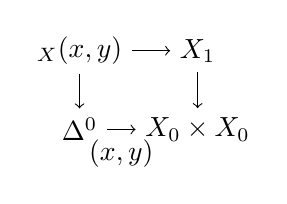
\begin{tikzpicture}[->]
      \node (downleft) at (0,0) {$\Delta^0$};
      \node (downright) at (1.5,0) {$X_0 \times X_0$};
      \node (upleft) at (0,1) {$\map_X(x,y)$};
      \node (upright) at (1.5,1) {$X_1$};
      % \node[below,right] (upleft) {$\mathrm{p.b.}$};
      \draw (downleft) -- node[below] {$(x,y)$} (downright);
      \draw (upleft) -- (downleft);
      \draw (upleft) -- (upright);
      \draw (upright) -- (downright);
    \end{tikzpicture}  
    \]
  \end{definition}

  Segal空間における射空間は「空間」である. 

  \begin{remark}
    Segal空間$X$の任意の対象$x,y$に対して, $\map_X(x,y)$はKan複体である. 
  \end{remark}

\end{frame}

\begin{frame}
  \frametitle{Segal空間における射の合成}

  Segal空間において, 射の合成は「可縮な空間の選択を除いて」一意に定まる. 

  \begin{lemma}
    Segal空間$X$の任意の対象$x_0,\cdots,x_n$に対して, 次の単体的集合の射
    \begin{align*}
      \map_X(x_0,\cdots,x_n) \to \map_X(x_0,x_1) \times \cdots \times \map_X(x_{n-1},x_n)
    \end{align*}
    は自明なKanファイブレーションである. 
  \end{lemma}

  \begin{definition}
    Segal空間$X$の射$f : x \to y, g : y \to z$に対して, 単体的集合$\comp(f,g)$を次のプルバックで定義する. 
    \[
    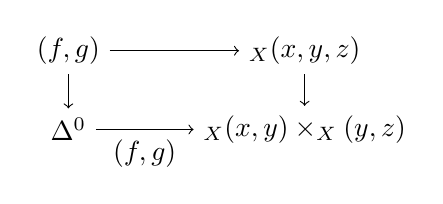
\begin{tikzpicture}[->]
      \node (downleft) at (0,0) {$\Delta^0$};
      \node (downright) at (3,0) {$\map_X(x,y) \times \map_X(y,z)$};
      \node (upleft) at (0,1) {$\comp(f,g)$};
      \node (upright) at (3,1) {$\map_X(x,y,z)$};
      % \node[below,right] (upleft) {$\mathrm{p.b.}$};
      \draw (downleft) -- node[below] {$(f,g)$} (downright);
      \draw (upleft) -- (downleft);
      \draw (upleft) -- (upright);
      \draw (upright) -- (downright);
    \end{tikzpicture}  
    \]
  \end{definition}

  \begin{remark}
    Segal空間$X$の射$f : x \to y, g : y \to z$に対して, $\comp(f,g)$は可縮なKan複体である.
  \end{remark}

\end{frame}

\begin{frame}
  \frametitle{Segal空間における射の合成}

  Segal空間において, 射の合成は「ホモトピーの違いを除いて」結合的かつ単位的である. 

  \begin{definition}[ホモトピック]
    $f, g : x \to y$をSegal空間$X$の射とする. 
    $f,g : \Delta^0 \to \map_X(x,y)$が単体的集合のホモトピックであるとき, $f$と$g$はホモトピック(homotopic)であるという. 
  \end{definition}

  \begin{theorem}
    合成可能な射の組$f,g,h$に対して, $(hg)f \sim h(gf)$かつ$f\id \sim f$, $\id f \sim f$である. 
  \end{theorem}

  \begin{definition}[ホモトピー同値の空間]
    Segal空間$X$に対して, ホモトピー同値のなす単体的部分集合を$X_\hoequiv \subset X_1$と表す. 
  \end{definition}

  % $\map_X(x,y)$におけるホモトピー類を用いて, Segal空間のホモトピー圏を定義する. 
  
  % \begin{definition}[ホモトピー圏]
  %   Segal空間$X$に対して, 小圏$\Ho(X)$を次のように定義し, $X$のホモトピー圏(homotopy category)という.
  %   \begin{itemize}
  %     \item $\Ho(X)$の対象は$X$の対象と同じ
  %     \item $\Ho(X)$の任意の対象$x,y$に対して, $\Hom_{\Ho(X)}(x,y)$は射空間のホモトピー類$\pi_0(\map_X(x,y))$
  %   \end{itemize}
  % \end{definition}

\end{frame}

\begin{frame}
  \frametitle{完備Segal空間}

  Segal空間において, 圏の性質とホモトピー論の性質は整合的ではない. 
  \footnote{
    walking isomorhismをもつ亜群$\{0 \leftrightarrow 1\}$と1点圏$\{\ast\}$を比較するとよい. 
  } 

  \begin{block}{}
    2つの対象が「Segal空間$X$においてホモトピックである」ことと, 「Kan複体$X_0$においてホモトピックである」ことを同値にする必要がある. 
  \end{block}

  \begin{definition}[完備Segal空間]
    Segal空間$X$に対して, 次の単体的集合の射
    \begin{align*}
      s_0 : X_0 \to X_\hoequiv
    \end{align*}
    がKan弱同値のとき, $X$は完備(complete)であるという. 
  \end{definition}

  完備性は, 圏論的な同型(対象の同型)とホモトピー論的な同値(ホモトピー同値)が1対1に対応するような条件である. 

  \begin{theorem}
    小圏$\C$に対して, 脈体$\N(\C)$が完備であることと, $\C$がgaunt
    \footnote{
      圏$\C$が恒等射以外の同型射を持たないとき, $\C$はgauntであるという. 
    }
    であることは同値である. 
  \end{theorem}

\end{frame}

% \section{$(\infty,1)$圏のモデル : 相対圏}

\begin{frame}
  \frametitle{相対圏}

  今まで見たように, $(\infty,1)$圏は圏論とホモトピー論の共通の一般化であった. 
  
  よって, ホモトピーの情報を「weak equivalenceの射のクラス」として持つような圏が考えられる. 

  \begin{definition}[相対圏]
    小圏$\C$と$\C$のwide部分圏
    \footnote{
      圏$\C$の対象をすべて含むような部分圏をwide部分圏という. 
    }
    $W$の組$(\C,W)$を相対圏(relative category)という. 
    
    % $W$の構造を保つような相対圏の関手を相対関手(relative functor)という. 
    % 相対圏と相対関手のなす圏を$\RelCat$と表す. 
  \end{definition}

  通常の圏は2つの極端な方法で相対圏とみなせる. 

  \begin{example}[極大と極小]
    $(\C,W)$を相対圏とする. 
    $W=\C$のとき, $(\C,W)$は極大(maximal)であるといい, $\C_\max$と表す. 

    $W$が恒等射以外の射を含まないとき, $(\C,W)$は極小(minimal)であるといい, $\C_\min$と表す.
  \end{example}

  相対圏の間のweak equivalenceを保つような関手を定義する. 

  \begin{definition}[相対関手]
    $(\C,W), (\C',W')$を相対圏とする. 
    関手$F : \C \to \C'$が$F(W) \subset W'$を満たすとき, $F$を相対関手(relative functor)という. 
  \end{definition}

  相対圏と相対関手のなす圏を$\RelCat$と表す. 
  相対半順序集合と相対関手のなす圏を$\RelPos$と表す. 

\end{frame}

\begin{frame}
  \frametitle{半順序集合の細分化}

  単体的集合の重心細分と同様に, 相対半順序集合の細分化を定義する. 

  \begin{definition}[終細分化]
    相対半順序集合$\P$に対して, 相対半順序集合$\xi_t\P$を次のように定義し, $\P$の終細分化(terminal subdivision)という. 
    \begin{itemize}
      \item $\xi_t\P$の対象は$\RelPos$におけるmono射$x : [n]_\min \to \P$ ($n \geq 0$)
      \item $\xi_t\P$の射は次の図式を可換にするような射$[n_1]_\min \to [n_2]_\min$
      \[
      \begin{tikzpicture}[,->]
        \node (upleft) at (0,0) {$[n_1]_\min$};
        \node (upright) at (2,0) {$[n_2]_\min$};
        \node (down) at (1,-1) {$\P$};
        \draw (upleft) -- (upright);
        \draw (upleft) -- node[left] {$x_1$} (down);
        \draw (upright) -- node[right] {$x_2$} (down);
      \end{tikzpicture}
      \]
      \item $\xi_t\P$のweak equivalenceは誘導される射$x_1(n_1) \to x_2(n_2)$が$\P$のweak equivalenceであるような射
    \end{itemize}
  \end{definition}

  終細分化を与える対応は関手$\xi_t : \RelPos \to \RelPos$を定める. 
  双対的に, 始細分化$\xi_i :  \RelPos \to \RelPos$も定義される. 

  \begin{definition}[2重細分化]
    相対半順序集合$\P$に対して, $\xi\P := \xi_t\xi_i\P$を$\P$の2重細分化(two-fold subdivion)という. 
  \end{definition}

\end{frame}

\section{モデル圏論}

\begin{frame}
  \frametitle{モデル圏とは}

  \begin{block}{モデル圏}
    モデル圏とは, 位相空間上のホモトピー論を抽象的に行うための枠組みである. 

    Quillenはホモトピー論を行うためにはweak equivalence, fibration, cofibrationの3つの射が重要であることを見抜き, この射の性質を公理化した. 

    これにより, 位相空間の圏以外でもホモトピー論が行うことができるようになった. 

    例えば, 位相空間のCW近似や複体のprojective resolutionが, モデル圏におけるコファイブラント置換によって説明できる. 
  \end{block}

  \begin{block}{Quillen同値}
    モデル圏$\M$に対して, ホモトピー圏$\Ho(\M)$が定義される. 
    
    モデル圏の同値として, Quillen同値がある. 
    この同値はモデル圏として随伴であって, ホモトピー圏が圏同値であるような条件である. 

    よって, $(\infty,1)$圏の理論のモデルが等価であるかは, 2つのモデル圏がQuillen同値であるかで判断する. 
  \end{block}

\end{frame}

\begin{frame}
  \frametitle{単体的集合の圏上のJoyalモデル構造}

  単体的集合の圏におけるweak equivalenceとして, Kan弱同値のほかにJoyal弱同値がある. 

  \begin{definition}[Joyal弱同値]
    $f : S \to T$を単体的集合の射とする.
    任意の擬圏$\C$に対して, 
    \begin{align*}
      \h\Fun(T,\C) \to \h\Fun(S,\C)
    \end{align*}
    が通常の圏同値のとき, $f$をJoyal弱同値(Joyal weak equivalence)
    \footnote{
      一般には, (弱)圏同値((weak) categorical equivalence)と呼ばれる. 
    }
    という. 
  \end{definition}

  ファイブラント対象がちょうど擬圏であるような$\sSet$上のモデル構造が存在する. 

  \begin{theorem}[Joyalモデル構造]
    単体的集合のmono射をcofibration, Joyal同値をweak equivalenceとするような, $\sSet$上のモデル構造が存在する. 

    このモデル構造を$\sSet$上のJoyalモデル構造といい, $(\sSet)_\Joyal$と表す. 
  \end{theorem}

  \begin{theorem}
    $(\sSet)_\Joyal$におけるファイブラント対象はちょうど擬圏である. 
  \end{theorem}

\end{frame}

\begin{frame}
  \frametitle{単体的空間の圏上のRezkモデル構造}

  \begin{definition}[Rezk弱同値]
    $f : X \to Y$を単体的空間の射とする. 
    任意の完備Segal空間$W$に対して, 
    \begin{align*}
      \Map_{\sSpace}(Y,W) \to \Map_{\sSpace}(X,W)
    \end{align*}
    がKan弱同値のとき, $f$をRezk弱同値(Rezk weak equivalence)という. 
  \end{definition}

  ファイブラント対象がちょうど完備Segal空間であるような$\sSpace$上のモデル構造が存在する. 

  \begin{theorem}[Rezkモデル構造]
    単体的空間のmono射をcofibration, Rezk弱同値をweak equivalenceとするような, $\sSpace$上のモデル構造が存在する. 

    このモデル構造を$\sSpace$上のRezkモデル構造といい, $(\sSpace)_\Rezk$と表す. 
    \footnote{
      一般には, $(\sSpace)_\Rezk$は$(\sSpace)_\Reedy$のBousfield局所化を用いて定義される. 
    }
  \end{theorem}

  \begin{theorem}
    $(\sSpace)_\Rezk$におけるファイブラント対象はちょうど完備Segal空間である. 
  \end{theorem}

\end{frame}

\begin{frame}
  \frametitle{相対圏の圏上のBarwick-Kanモデル構造}

  随伴によってモデル構造がリフトされる. 
  この定理を用いて, 相対圏の圏上のモデル構造を定義する. 

  \begin{theorem}
    $\C$をコファイブラント生成なモデル圏, $F: \C \rightleftarrows \D : G$を随伴とする. 
    $(F,G)$がいい条件を満たすとき, 次のような$\D$上のモデル構造が存在する. 
    \begin{itemize}
      \item weak equivalenceは$G$での像が$\C$におけるweak equivalenceとなるような$\D$の射
      \item fibrationは$G$での像が$\C$におけるfibrationとなるような$\D$の射
    \end{itemize}
  \end{theorem}

  随伴$(N_\xi,K_\xi)$を用いて, $(\sSpace)_{\Reedy}$から$\RelCat$上にモデル構造をリフトすることができる. 

  \begin{theorem}[Barwick-Kanモデル構造]
    $N_\xi$の像がReedy弱同値である相対関手をweak equivalence, $N_\xi$の像がReedyファイブレーションであるような相対関手をfibrationとするような, $\RelCat$上のモデル構造が存在する. 

    このモデル構造を$\RelCat$上のBarwick-Kanモデル構造といい, $(\RelCat)_\BK$と表す. 
  \end{theorem}

\end{frame}

\section{$(\infty,1)$圏の理論のモデルの等価性}

\begin{frame}
  \frametitle{位相的圏と単体的圏の等価性}

  幾何学的実現と特異単体の随伴は豊穣圏の間の随伴にリフトする. 

  \begin{remark}
    随伴$|-| : \sSet \rightleftarrows \Top : \Sing$は, 随伴$|-| : \Cat_\Delta \rightleftarrows \Cat_{\Top} : \Sing$を定める. 
  \end{remark}

  本質的には次の命題から従う. 

  \begin{theorem}
    いいモノイダルモデル圏のQuillen随伴$F: \bfA \rightleftarrows \bfA' : G$は, Quillen随伴$F: (\Cat_{\bfA})_\Berg \leftrightarrows (\Cat_{\bfA'})_\Berg : G$を定める. 
    
    更に, Quillen同値からはQuillen同値が定まる. 
  \end{theorem}

  $\Cat_\Delta$と$\Cat_{\Top}$はBergnerモデル構造としてQuillen同値である. 

  \begin{theorem}[\cite{Ber07}]
    随伴$|-| : \Cat_\Delta \rightleftarrows \Cat_{\Top} : \Sing$は次のQuillen同値を定める. 
    \begin{align*}
      |-| : (\Cat_\Delta)_\Berg \rightleftarrows (\Cat_{\Top})_\Berg : \Sing
    \end{align*}
  \end{theorem}

\end{frame}

\begin{frame}
  \frametitle{擬圏と位相的圏の等価性}

  $\sSet$と$\Cat_\Delta$の随伴をKan拡張を用いて構成する. 

  \begin{remark}
    関手$\mathfrak{C}[\Delta^-] : \Delta \to \Cat_\Delta$を$\mathfrak{C}[\Delta^-]([n]) := \mathfrak{C}[\Delta^n]$で定義する. 
    Kan拡張から, 次の随伴$(\mathfrak{C},\mathfrak{N})$が得られる. 
    \[
    \begin{tikzpicture}[->]
      \node (0) at (0,0) {$\Delta$};
      \node (1) at (1.5,0) {$\Cat_\Delta$};
      \node (2) at (0,1.5) {$\sSet$};
      \draw (0) -- node[below] {$\mathfrak{C}[\Delta^-]$} (1);
      \draw (0) -- node[left] {よ} (2);
      \draw (1) to[bend left=15] node[below] {$\mathfrak{N}$} (2);
      \draw (2) to[bend left=15] node[above] {$\mathfrak{C}$} (1);
    \end{tikzpicture}  
    \]
  \end{remark}

  \begin{theorem}[\cite{Ber07b}]
    随伴$\mathfrak{C} : \sSet \rightleftarrows \Cat_\Delta : \mathfrak{N}$は次のQuillen同値を定める. 
    \begin{align*}
      \mathfrak{C} : (\sSet)_\Joyal \rightleftarrows (\Cat_\Delta)_\Berg : \mathfrak{N}
    \end{align*}
  \end{theorem}

\end{frame}

\begin{frame}
  \frametitle{完備Segal空間と擬圏の等価性}

  $\sSpace$と$\sSet$の随伴をKan拡張を用いて構成する. 

  \begin{remark}
    $[n]$により自由生成される亜群の脈体を$\Delta'[n]$と表す. 
    関手$t : \Delta \times \Delta \to \sSet$を$t([m],[n]) := \Delta[m] \times \Delta'[n]$で定義する. 

    Kan拡張から, 次の随伴$(t_!,t^!)$が得られる. 
    \[
    \begin{tikzpicture}[->]
      \node (0) at (0,0) {$\Delta \times \Delta$};
      \node (1) at (1.5,0) {$\sSet$};
      \node (2) at (0,1.5) {$\sSpace$};
      \draw (0) -- node[below] {$t$} (1);
      \draw (0) -- node[left] {よ} (2);
      \draw (1) to[bend left=15] node[below] {$t^!$} (2);
      \draw (2) to[bend left=15] node[above] {$t_!$} (1);
    \end{tikzpicture}  
    \]
  \end{remark}

  \begin{theorem}[\cite{JT07}]
    随伴$(t_!,t^!)$は次のQuillen同値を定める.
    \begin{align*}
      t_! : (\sSpace)_\Rezk \rightleftarrows (\sSet)_\Joyal : t^!
    \end{align*}
  \end{theorem}

\end{frame}

\begin{frame}
  \frametitle{完備Segal空間と相対圏の等価性}

  $\sSpace$と$\RelCat$の随伴をKan拡張を用いて構成する.

  \begin{remark}
    関手$[-]^\xi_{\mathrm{m,m}} : \Delta \times \Delta \to \RelCat$を$[-]^\xi_{\mathrm{m,m}}([n],[m]):=\xi([n]_\min \times [m]_\max)$で定義する. 
    
    Kan拡張から, 次の随伴$(K_\xi,N_\xi)$が得られる. 
    \[
      \begin{tikzpicture}[->]
        \node (0) at (0,0) {$\Delta \times \Delta$};
        \node (1) at (1.5,0) {$\RelCat$};
        \node (2) at (0,1.5) {$\sSpace$};
        \draw (0) -- node[below] {$[-]^\xi_{\mathrm{m,m}}$} (1);
        \draw (0) -- node[left] {よ} (2);
        \draw (1) to[bend left=15] node[below] {$N_\xi$} (2);
        \draw (2) to[bend left=15] node[above] {$K_\xi$} (1);
      \end{tikzpicture}  
      \]
  \end{remark}

  \begin{theorem}[\cite{BK11}]
    随伴$(K_\xi,N_\xi)$は次のQuillen同値を定める.
    \begin{align*}
      K_\xi : (\sSpace)_{\Rezk} \rightleftarrows (\RelCat)_{\BK} : N_\xi
    \end{align*}
  \end{theorem}

\end{frame}

\begin{frame}
  \frametitle{まとめ}

  本稿で紹介したQuillen同値をまとめる. 

  \begin{block}{}
    次のQuillen同値の列が存在する. (上矢印が左Quillen同値)
    \[
    \begin{tikzpicture}
      \node (0) at (0,0) {$(\RelCat)_{\BK}$};
      \node (1) at (2.5,0) {$(\sSpace)_{\Rezk}$};
      \node (2) at (5,0) {$(\sSet)_{\Joyal}$};
      \node (3) at (7.5,0) {$(\Cat_\Delta)_{\Berg}$};
      \node (4) at (10,0) {$(\Cat_{\Top})_{\Berg}$};
      \draw[->] (0) to[bend right=15, yshift=-0.5ex] node[below] {$N_\xi$} (1);
      \draw[->] (1) to[bend right=15, yshift=0.5ex] node[above] {$K_\xi$} (0);
      \draw[->] (1) to[bend left=15, yshift=0.5ex] node[above] {$t_!$} (2);
      \draw[->] (2) to[bend left=15, yshift=0.5ex] node[below] {$t^!$} (1);
      \draw[->] (2) to[bend left=15, yshift=-0.5ex] node[above] {$\mathfrak{C}$} (3);
      \draw[->] (3) to[bend left=15, yshift=0.5ex] node[below] {$\mathfrak{N}$} (2);
      \draw[->] (3) to[bend left=15, yshift=-0.5ex] node[above] {$|-|$} (4);
      \draw[->] (4) to[bend left=15, yshift=0.5ex] node[below] {$\Sing$} (3);
    \end{tikzpicture}  
    \]
  \end{block}

\end{frame}

\begin{frame}[allowframebreaks]
  \frametitle{参考文献}

  \scriptsize
  \beamertemplatetextbibitems
  \bibliographystyle{apalike}
  \bibliography{tudoi5_cf}

\end{frame}


\end{document}